\chapter{Numerical Results}
\label{Numerical Results}

In this chapter, we will present some numerical studies concerning simulations with the random walk Metropolis~(RWM) algorithm and the Metropolis adjusted Langevin algorithm~(MALA). A simple simulation tool was implemented in python and was used to generate the following figures. We will briefly describe some properties like the estimation of integrated autocorrelation time to avoid ambiguousness. Also the different target distributions are described which are used for the simulations. Mainly, we want to verify that the theoretical and asymptotical results hold for finite dimensions~$N$. This is reached by performing simulations with RWM and MALA applied to several target distributions. Afterwards, these simulations are analyzed to measure the complexity and to find the optimal scaling (of the proposal variance) depending on $N$.
Further numerical studies concerning the optimal scaling of Metropolis-Hastings methods and in particular the RWM and MALA algorithm, can be found in~\autocite{Beskos2008, Gelman1996, Roberts2001}.

\section{Measuring Complexity: Integrated Autocorrelation Time}
\label{NR-integrated autocorrelation time}

In this section, we will present briefly the used measure of complexity. As introduced in Chapter~\ref{CC:Criteria}, there exist no uniqe and best criteria to ascertain a good performance of a (Markov) chain and hence, a Metropolis-Hastings method. In this section, we introduce the \textit{integrated autocorrelation time}, or more precisely, an suitable estimator for this quantity..

\section{Examples and Simulations}

\subsection{A Multimodal Example}

For instance, consider a $N$-dimensional bimodal target density of the form
\begin{equation}
 \label{NR-multimodal}
 \pi^{N} = \tfrac{1}{2} \; \mathcal{N}(-\mu_N, I_N ) +  \tfrac{1}{2} \; \mathcal{N}(\mu_N, I_N ),
\end{equation}
where $\mu_N = (m_N, 0, \dots, 0) \in \mathbb{R}^N$. The mass of this distribution is centered in the two modes~$-\mu_N$ and $\mu_N$. Although, this is the sum of two simpe $N$-dimensional Gaussians, the bimodal distribution is wether of i.i.d.\,product form nor of a scaled product form as defined in~(\ref{CC:iid product targets} and~(\ref{CC:Scaled product targets}), respectively. Indeed, the first coordinate is not merely a rescaling of the other coordinates. 

\begin{figure}%[htb]
 \begin{center} 
  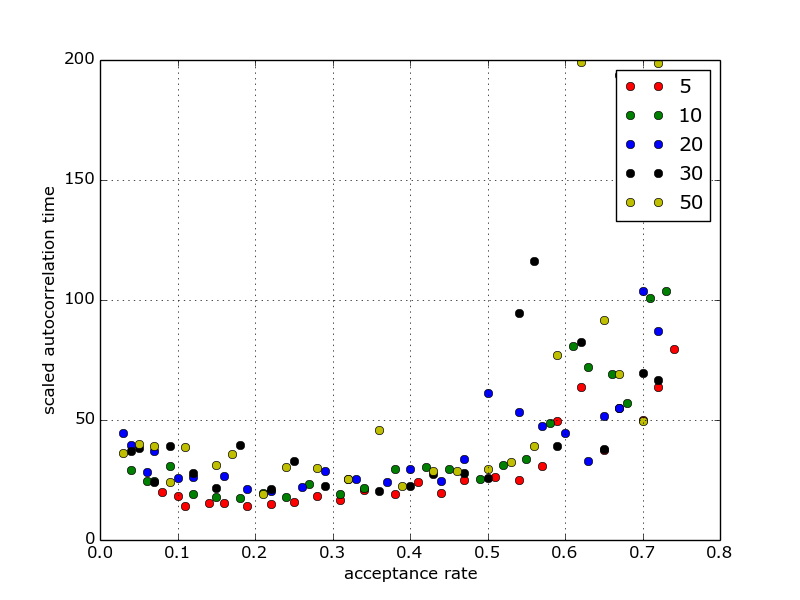
\includegraphics[width=0.83\textwidth]{RWM_ScaledAutocorrelationsDiagramm_MultimodalGaussian-m=2}
  \vspace*{1mm}
  \subcaption{The optimal scaling of RWM methods is achieved for acceptance rates near 0.234.}
  \label{fig:OptimalScaling-RWM-dimensions}
  \vspace*{3mm}
  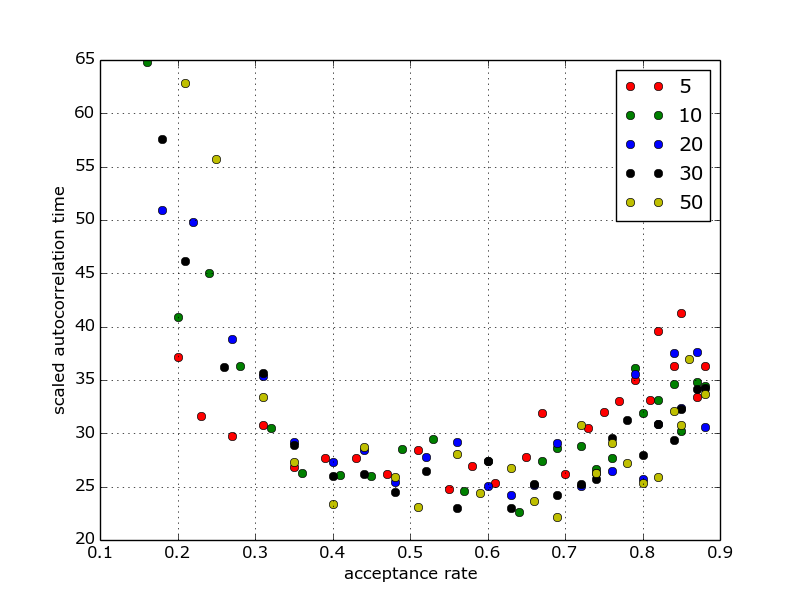
\includegraphics[width=0.83\textwidth]{MALA_ScaledAutocorrelationsDiagramm_MultimodalGaussian-m=2}
  \vspace*{1mm}
  \subcaption{The optimal scaling of MALA methods is achieved for acceptance rates near 0.574.}
  \label{fig:OptimalScaling-MALA-dimensions}
 \end{center}
  \caption{Plotted integrated autocorrelation time for different acceptance rates and various dimensions for a multimodal Gaussian target.}
  \label{fig:OptimalScaling for RWM and MALA in various dimensions}
\end{figure}

A numerical study for $m_N = 2$ for the RWM and MALA is illustrated in Figure~\ref{fig:OptimalScaling for RWM and MALA in various dimensions}. For each dimension $N \in \{ 5, 10, 20, 30, 50 \}$, several simulations of the RWM and MALA applied to the target~(\ref{NR-multimodal}) are performed. For different average acceptance rates, the scaled integrated autocorrelation time is calculated according to Section~\ref{NR-integrated autocorrelation time}. Several facts are well illustrated:
\begin{enumerate}
 \item Best performance of RWM near an acceptance rate of 0.234 and of MALA near an acceptance rate of 0.573. Hence, asymptotic results seem to apply for finite dimensional setting ($N \geq 5$).
 \item To reach optimality, it suffices to scale the simulation such that the average acceptance rate is near the optimal values of 0.234 and 0.574. The performance of RWM is good for an average acceptance rate in the intervall $[0.1, 0.4]$ and the MALA performs well for $[0.4, 0.75]$.
 \item It is not surprising, that the MALA algorithm has in practice a lower scaled integrated autocorrelation time as the theoretical complexity is better in comparison to the RWM algorithm due to the gradient information in the proposal of MALA algorithm.
\end{enumerate}

\begin{rem}
 The gradient~$\nabla \log \pi^{N}$ in the MALA algorithm can be numerically approximated by finite differences. Moreover, for both methods, a parallelization for high dimensions is possible. As only the acceptance and rejection steps requires all information on the actual position and the possible candidate, once per iteration, a spreading of information is sufficent.
\end{rem}
